\documentclass[12pt]{article}
\usepackage[utf8]{inputenc}

% Default fixed font does not support bold face
\DeclareFixedFont{\ttb}{T1}{txtt}{bx}{n}{12} % for bold
\DeclareFixedFont{\ttm}{T1}{txtt}{m}{n}{12}  % for normal

% Custom colors
\usepackage{color}
\definecolor{deepblue}{rgb}{0,0,0.5}
\definecolor{deepred}{rgb}{0.6,0,0}
\definecolor{deepgreen}{rgb}{0,0.5,0}
\setlength{\parskip}{2pt}%
\setlength{\parindent}{0pt}%
\usepackage{enumitem, amsmath, graphicx, wrapfig, float, nccmath, verbatim, fancyvrb, geometry, changepage, listings}
\usepackage[export]{adjustbox}
\newcommand\pythonstyle{\lstset{
		language=Python,
		basicstyle=\ttm,
		otherkeywords={self},             % Add keywords here
		keywordstyle=\ttb\color{deepblue},
		emph={MyClass,__init__},          % Custom highlighting
		emphstyle=\ttb\color{deepred},    % Custom highlighting style
		stringstyle=\color{deepgreen},
		frame=tb,                         % Any extra options here
		showstringspaces=false            % 
}}


% Python environment
\lstnewenvironment{python}[1][]
{
	\pythonstyle
	\lstset{#1}
}
{}

% Python for external files
\newcommand\pythonexternal[2][]{{
		\pythonstyle
		\lstinputlisting[#1]{#2}}}

% Python for inline
\newcommand\pythoninline[1]{{\pythonstyle\lstinline!#1!}}
\title{%
	ECE-471 Selected Topics in Machine Learning \\
	Prof. Curro \\
	Midterm Project}
\author{Evan Bubniak, Zhang Jinhan}
\begin{document}
\maketitle

\section{Results}

\begin{figure}[H]
	\centering
	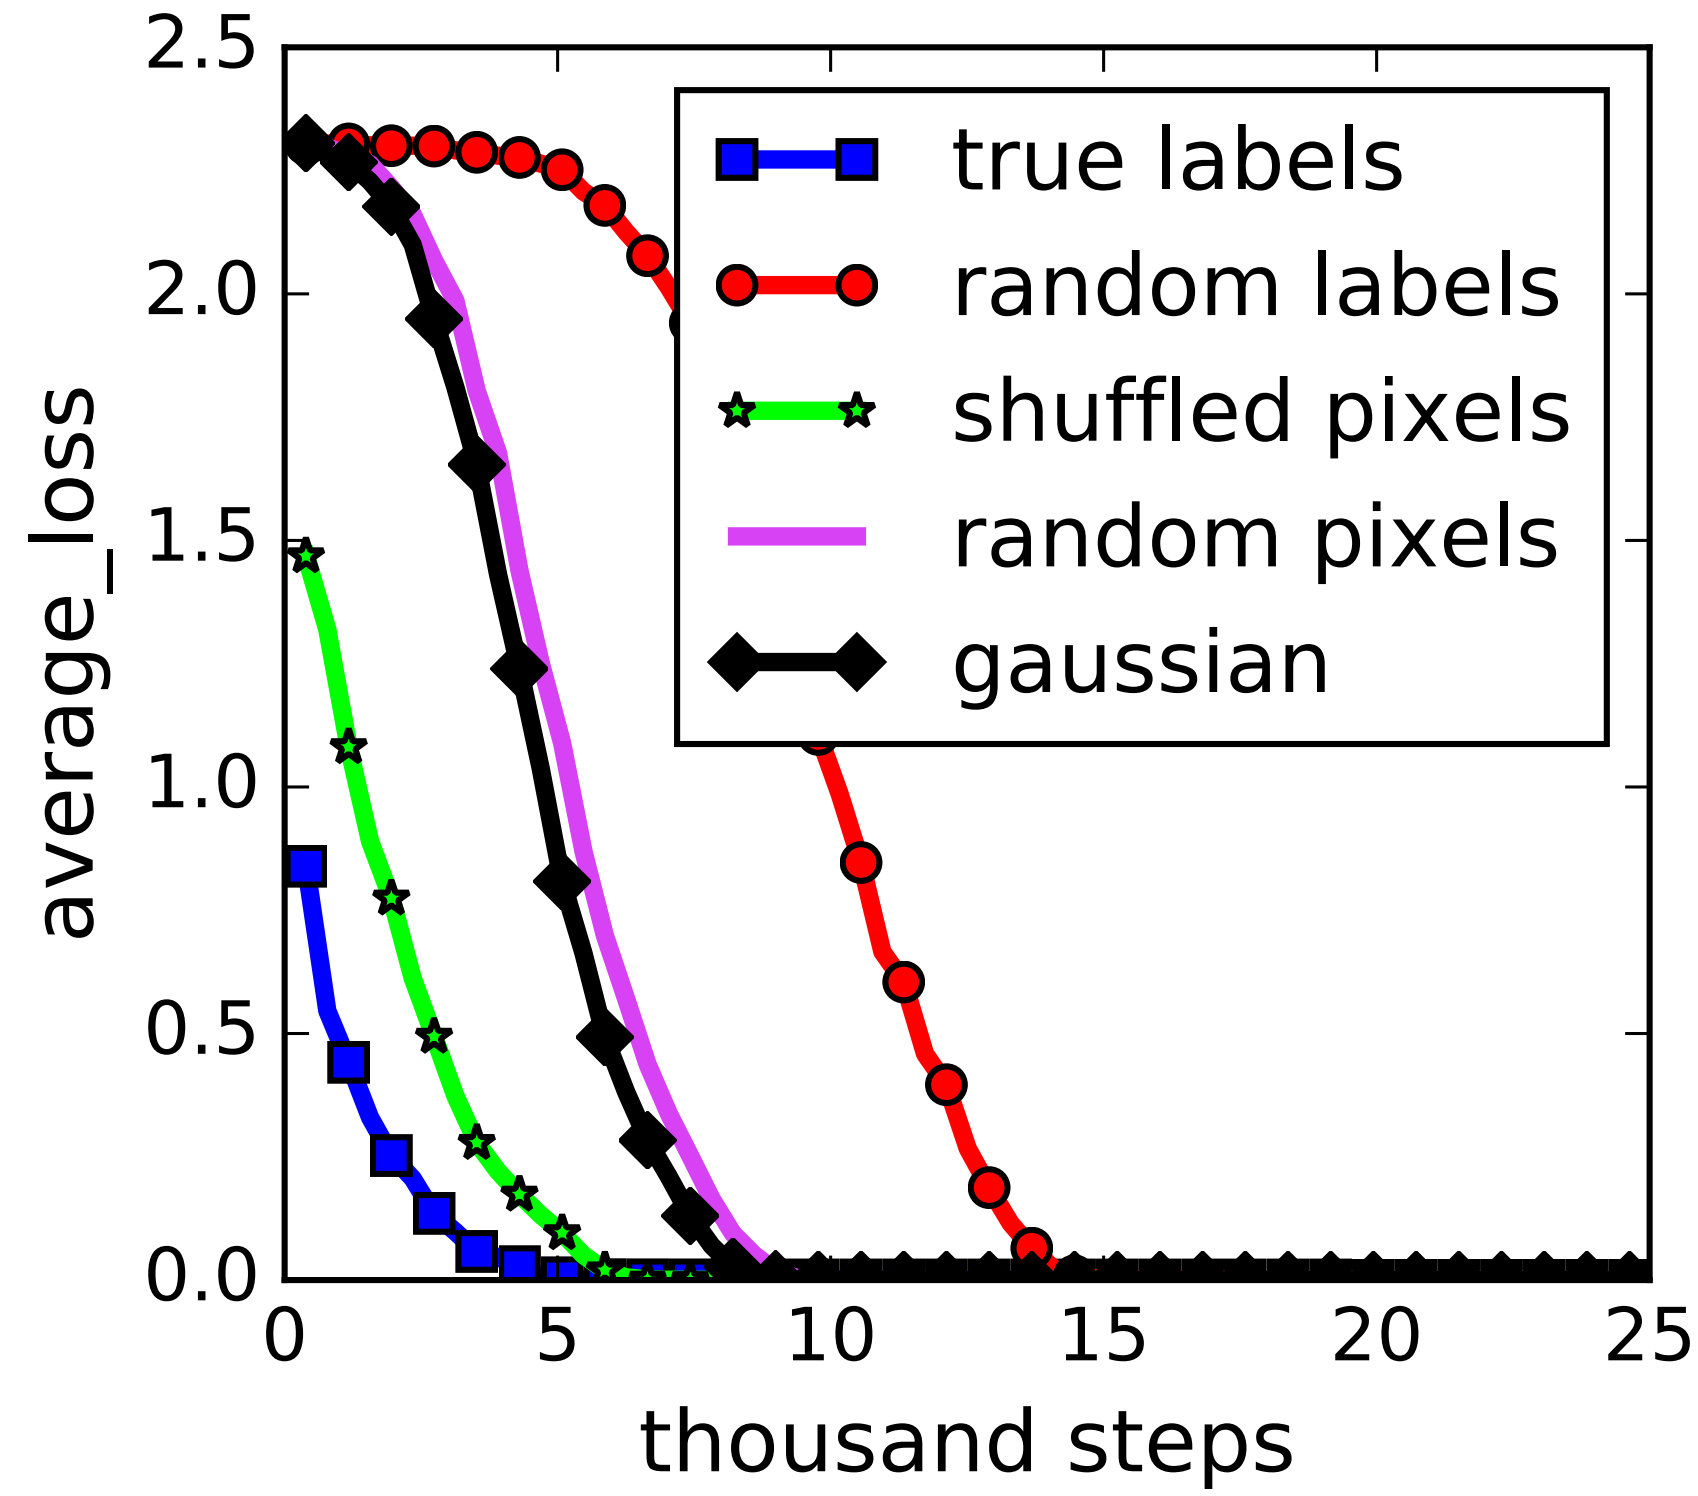
\includegraphics[width=0.75\textwidth]{paper_source/fig.png}
	\caption{Juxtaposition of the noisy data points, the noiseless sinewave they are based on, and the manifold of the stochastic gradient descent regression model.}
\end{figure}

\begin{figure}[H]
	\centering
	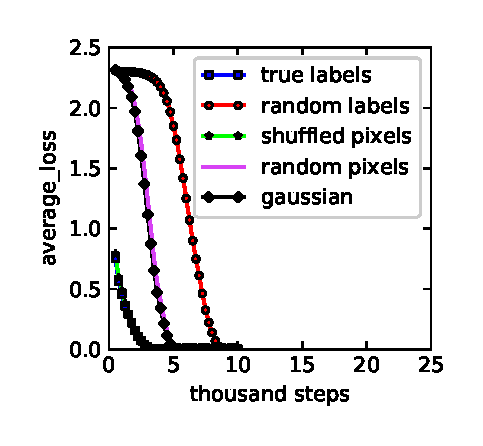
\includegraphics[width=0.75\textwidth]{results_1/output.eps}
	\caption{A plot of each of the basis functions, with the weights and intercept removed.}
\end{figure}

\clearpage
\begin{adjustwidth}{-50pt}{0pt}

\section{Code}
\pythonexternal{main.py}
\end{adjustwidth}

\end{document}